\documentclass[10pt,a4paper]{scrreprt}
\usepackage[utf8x]{inputenc}
\usepackage[ngerman]{babel}
\usepackage[T1]{fontenc}
\usepackage{amsmath}
\usepackage{amsfonts}
\usepackage{amssymb}
\usepackage{graphicx}
\usepackage{titlepic}
\usepackage{hyperref}
\hypersetup{
	colorlinks=false
}
\usepackage{float}
\usepackage{tabu}
\usepackage{longtable}
\usepackage{color}

\definecolor{sehrGut     }{rgb}{.000,.678,.000}
\definecolor{gut         }{rgb}{.490,.651,.278}
\definecolor{okay        }{rgb}{.678,.655,.624}
\definecolor{schlecht    }{rgb}{.863,.137,.000}
\definecolor{sehrSchlecht}{rgb}{1   ,.000,.000}

\newcommand*{\sehrGut     }{\textcolor{sehrGut     }{\textbf{Sehr Gut}}}
\newcommand*{\gut         }{\textcolor{gut         }{\textbf{Gut}}}
\newcommand*{\okay        }{\textcolor{okay        }{\textbf{Okay}}}
\newcommand*{\schlecht    }{\textcolor{schlecht    }{\textbf{Schlecht}}}
\newcommand*{\sehrSchlecht}{\textcolor{sehrSchlecht}{\textbf{Sehr Schlecht}}}

\title{Projekthandbuch}
\titlepic{
\includegraphics[width=0.3\textwidth]{images/lindale-logo}}
\subtitle{v1.2.5}
\author{Jeremias Eppler, Jochen Morent, Georgi Georgiev}
\begin{document}
\maketitle
\tableofcontents
%-----------------------------------------------
%  Projektstart
%-----------------------------------------------
\newpage
\chapter{Projektstart}
	\section{Projekt-Kontext-Beziehungen}
		\subsection{Zeitlicher Kontext}
\begin{figure}[!ht]
\center
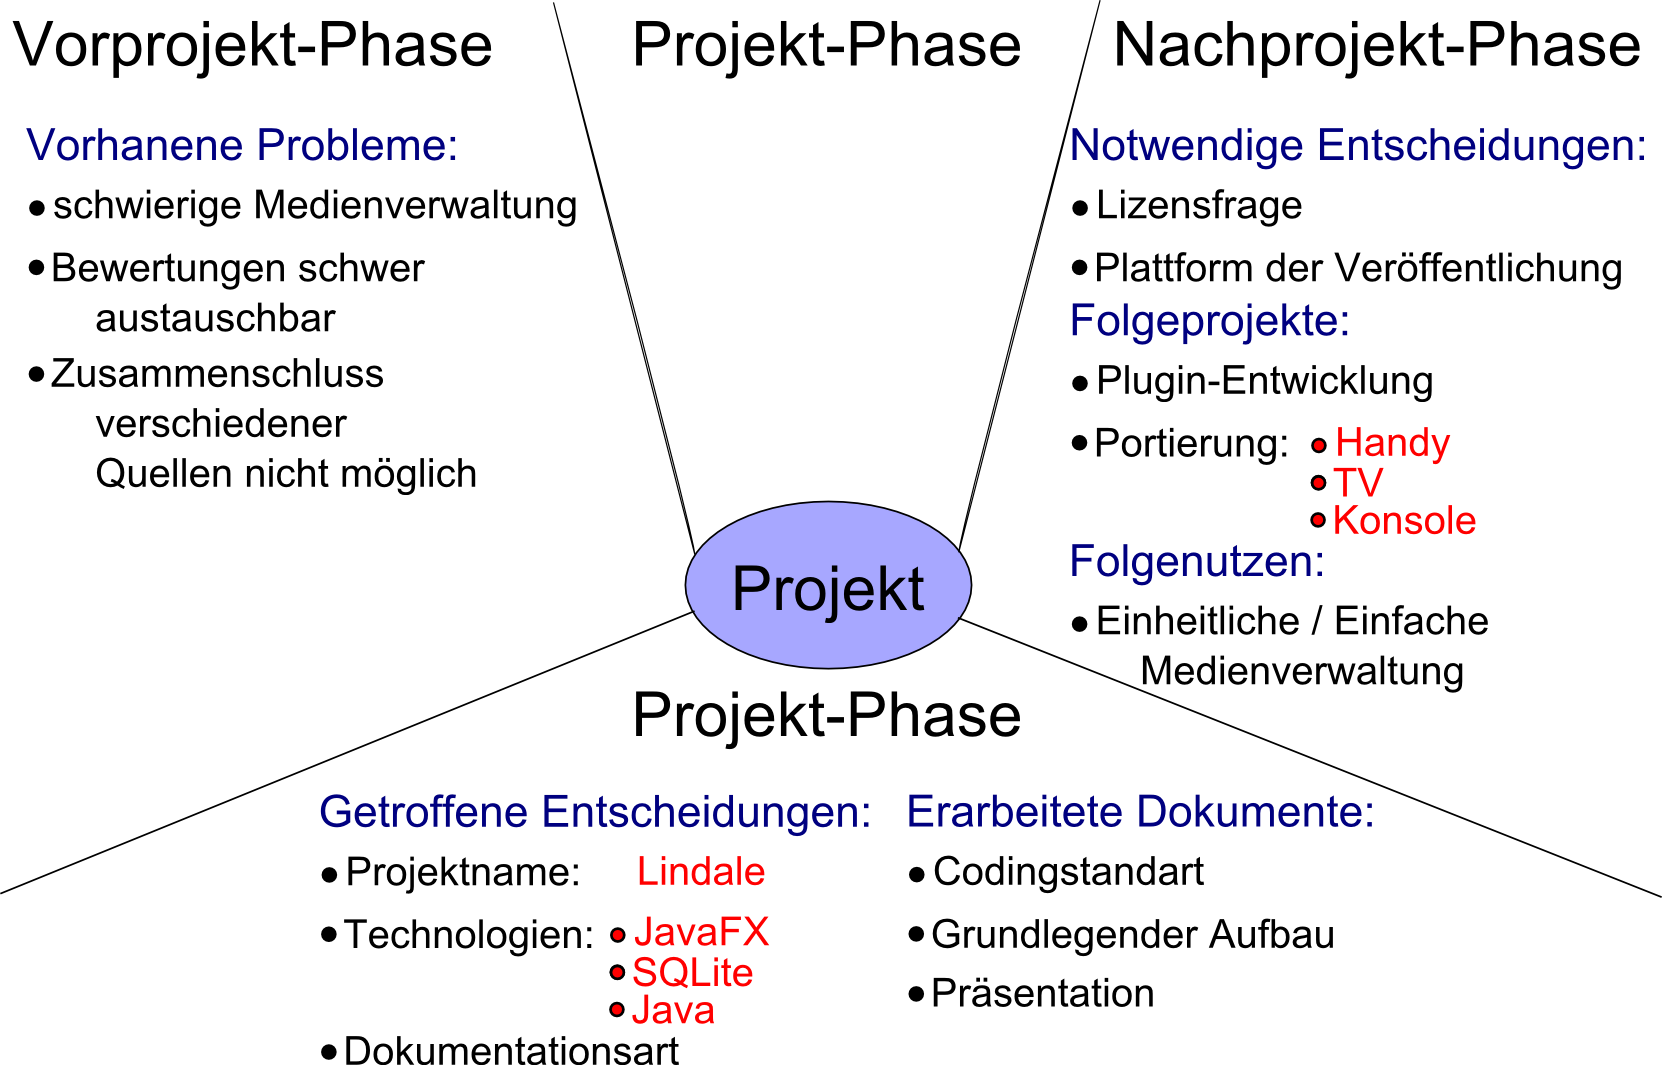
\includegraphics[width=\linewidth]{images/zeitlicher-kontext}
\caption{Zeitlicher Kontext}
\end{figure}
		\newpage
		\subsection{Sachlicher Kontext}
\begin{figure}[!ht]
\center
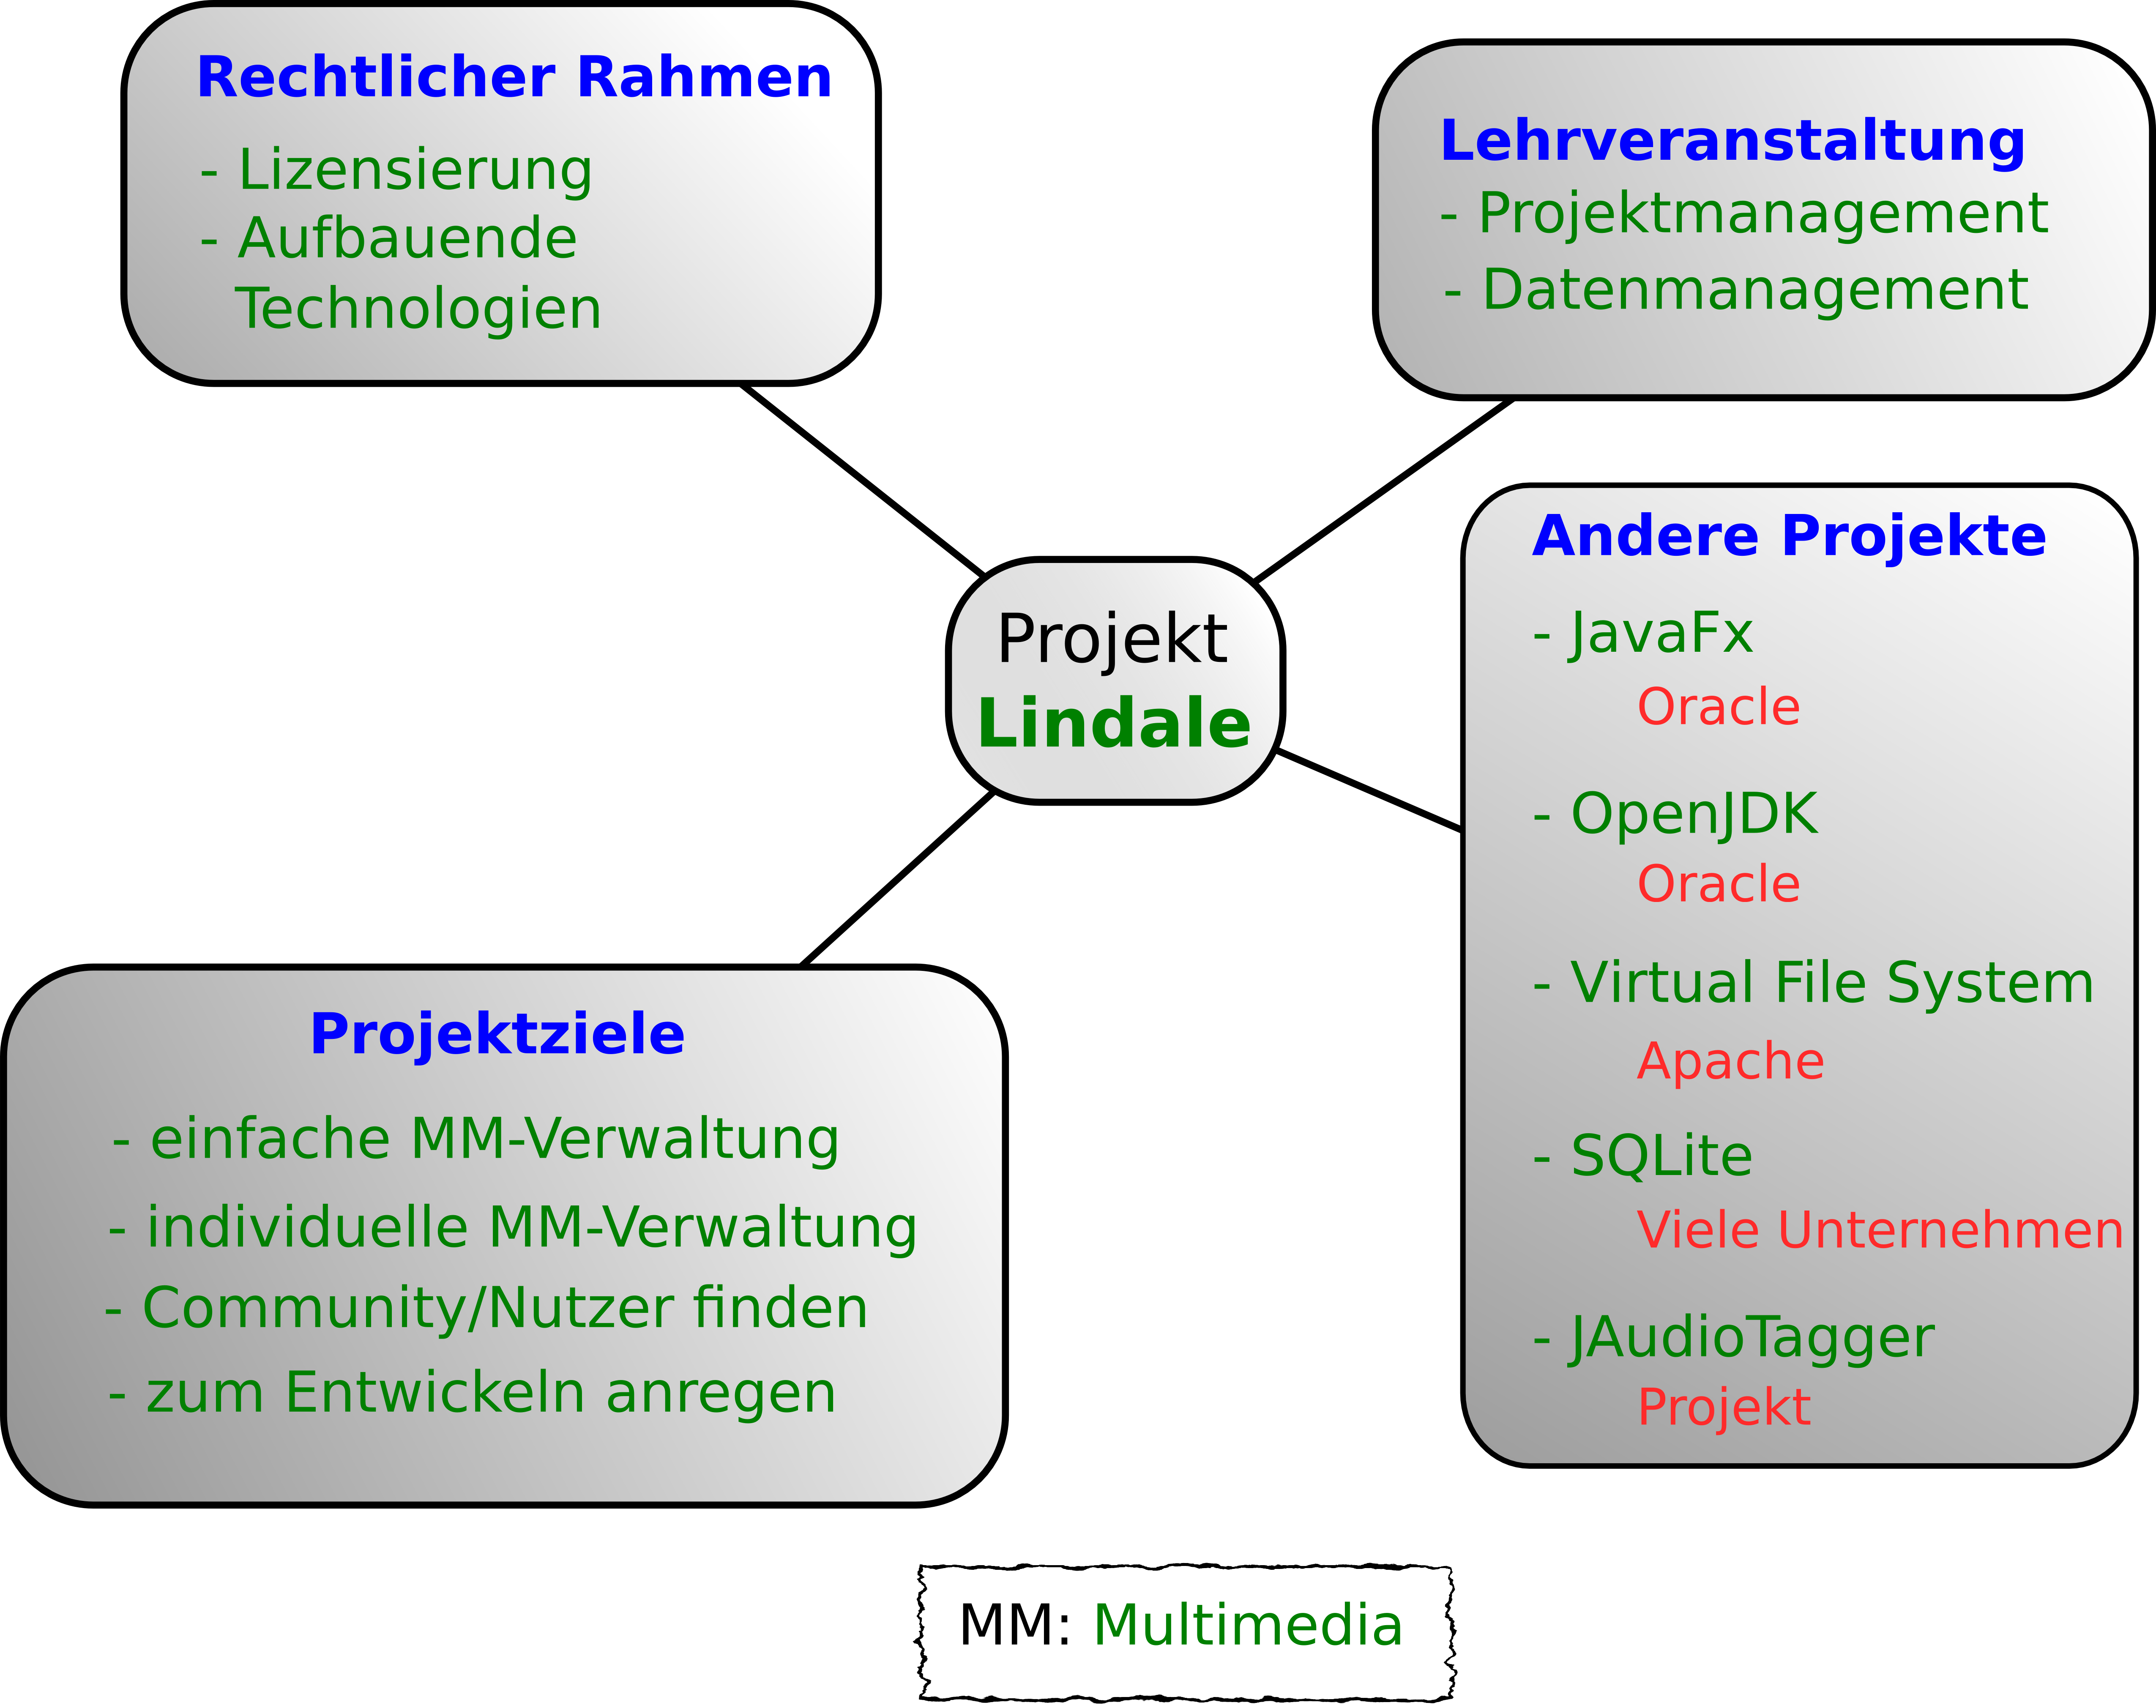
\includegraphics[width=\linewidth]{images/sachlicher-kontext}
\caption{Sachlicher Kontext}
\end{figure}
		\newpage
		\subsection{Sozialer Kontext}
\begin{figure}[!ht]
\center
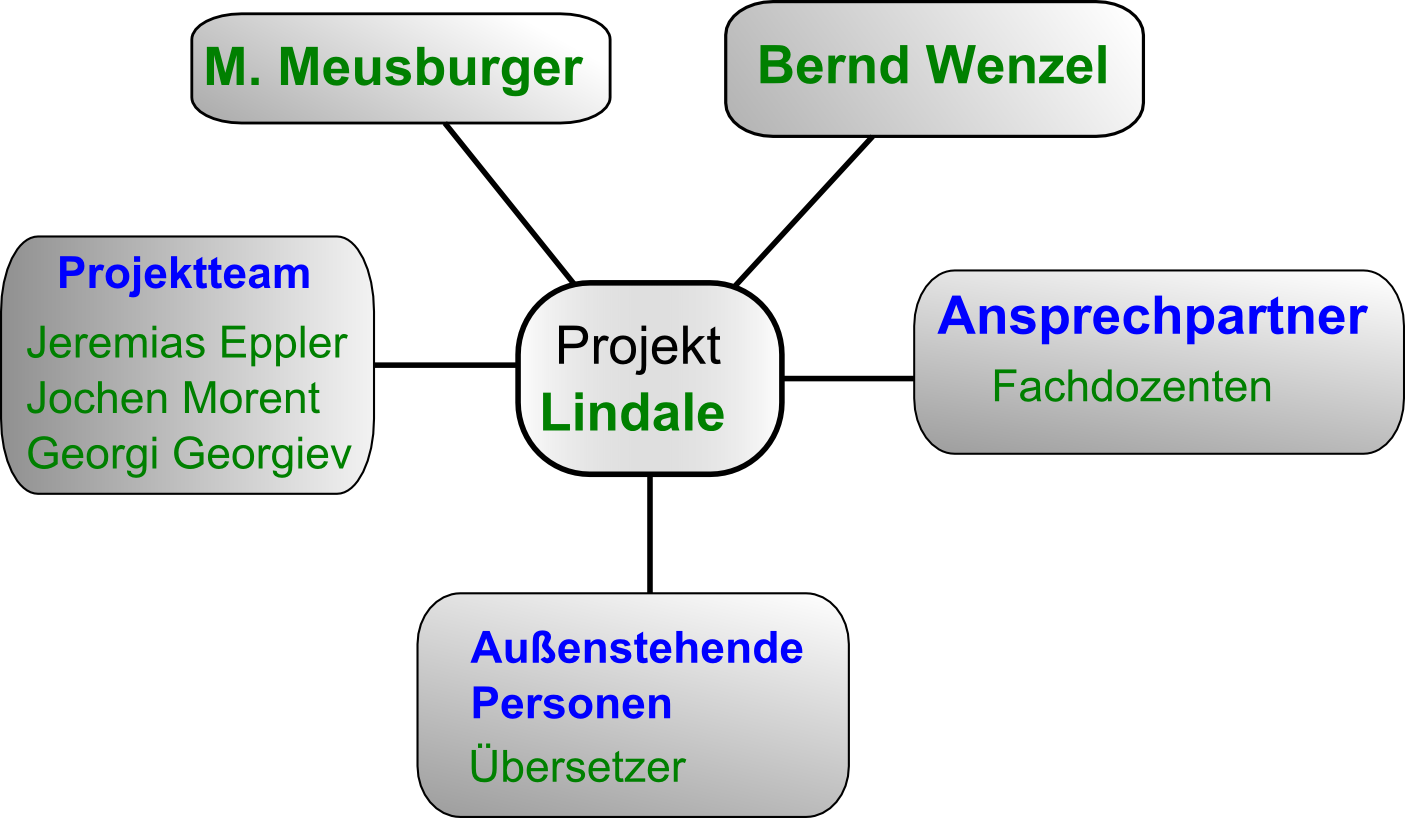
\includegraphics[width=\linewidth]{images/sozialer-kontetxt}
\caption{Sozialer Kontext}
\end{figure}
	\clearpage
	\section{Projektauftrag}
\tabulinesep=1.3mm
\begin{longtabu} to 14cm {|X[l]|X[l]|X[l]|X[l]|}
\hline
\parbox{3cm}{Projektstartereignis:} & \parbox{3cm}{Anfang der Recherche} & \parbox{3cm}{Projektstarttermin:} & \parbox{3cm}{03.10.2013} \\
\hline
\parbox{3cm}{Projektendereignis:} & \parbox{3cm}{Präsentation des Projekts} & \parbox{3cm}{Projektendtermin:} & \parbox{3cm}{10.01.2014} \\
\hline
\parbox{3cm}{Projektziele:} & \parbox{3cm}{
Verbessertes Medien-Verwaltungs-Tool\\ \\
Vereinheitlichte Medienverwaltung
} & \parbox{3cm}{Nicht-Projektziele:} & \parbox{3cm}{
Keine Backup-Lösung\\ \\
Weder logische noch physische Speicherung wird verwaltet
} \\
\hline
\parbox{3cm}{Hauptaufgabe:} & \multicolumn{3}{l|}{\parbox{8cm}{Planen, implementieren und testen des Hauptprogrammes und der Datenbank}} \\
\hline
\parbox{3cm}{Projektauftraggeber:} & \parbox{3cm}{Projektteam und B. Wenzel} & \parbox{3cm}{Projektleiter:} &  \parbox{3cm}{Jochen Morent} \\
\hline
\parbox{3cm}{Projektteam-\\mitglieder:} & \multicolumn{3}{l|}{\parbox{8cm}{
Jochen Morent \\
Jeremias Eppler \\
Geogie Georgiev}} \\
\hline
\parbox{3cm}{Version: 1.0} & \parbox{3cm}{Datum: 06.01.2014} & \parbox{3cm}{Ersteller:Jochen Morent} &\\
\hline
\end{longtabu}

	\clearpage
	\section{Ziele und Objekte}
		\subsubsection{Hauptziele}

\begin{itemize}
	\item Verbessertes Medien-Verwaltungs-Tool
	\item Vereinheitlichte Medienverwaltung
\end{itemize}
\subsubsection{Nebenziele}
\begin{itemize}
	\item Bewertungssystem
	\item Arbeiten mit Datenbaken
	\item Einarbeiten in JavaFX
	\item Arbeiten mit APIs
\end{itemize}
\subsubsection{Nichtziele}
\begin{itemize}
	\item Keine Backup-Lösung
	\item Weder logische noch physische Speicherung wird verwaltet
\end{itemize}
\subsubsection{Objekte}
\begin{itemize}
	\item Projektdokumentation
	\item Datenbankentwurf (Datenbank/Modelierung)
	\item UML-Diagramme (Klasse/Sequenz)
	\item Plugin-Manager (Manager/PluginAPI)
	\item Plugins
	\item APIs
	\item Ressourcen-Sammlung
	\item GUI-Entwurf/-Modell
\end{itemize}
	\clearpage
	\section{Projektorganisation}
		\subsection{Projektorganigram}
\begin{figure}[!ht]
\center
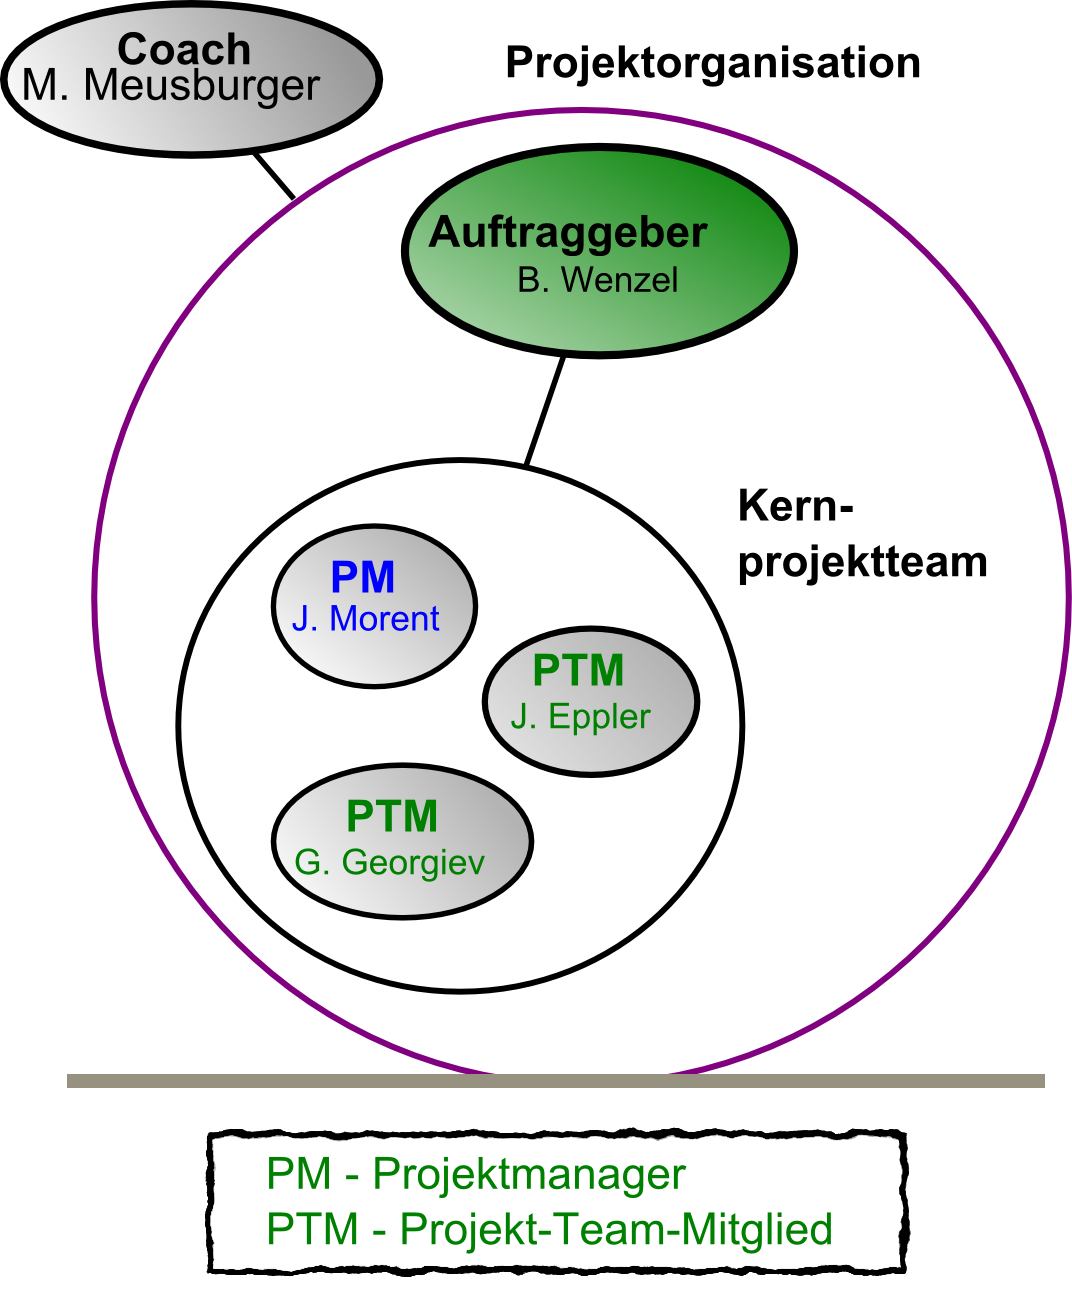
\includegraphics[width=.7\textwidth, height=.7\textheight, keepaspectratio, angle=0]{images/projektorganisation}
\caption{Projektorganisation}
\end{figure}
	\clearpage
	\section{Projektleistungsplan}
		\subsection{Projektstrukturplan}
\begin{figure}[!ht]
\center
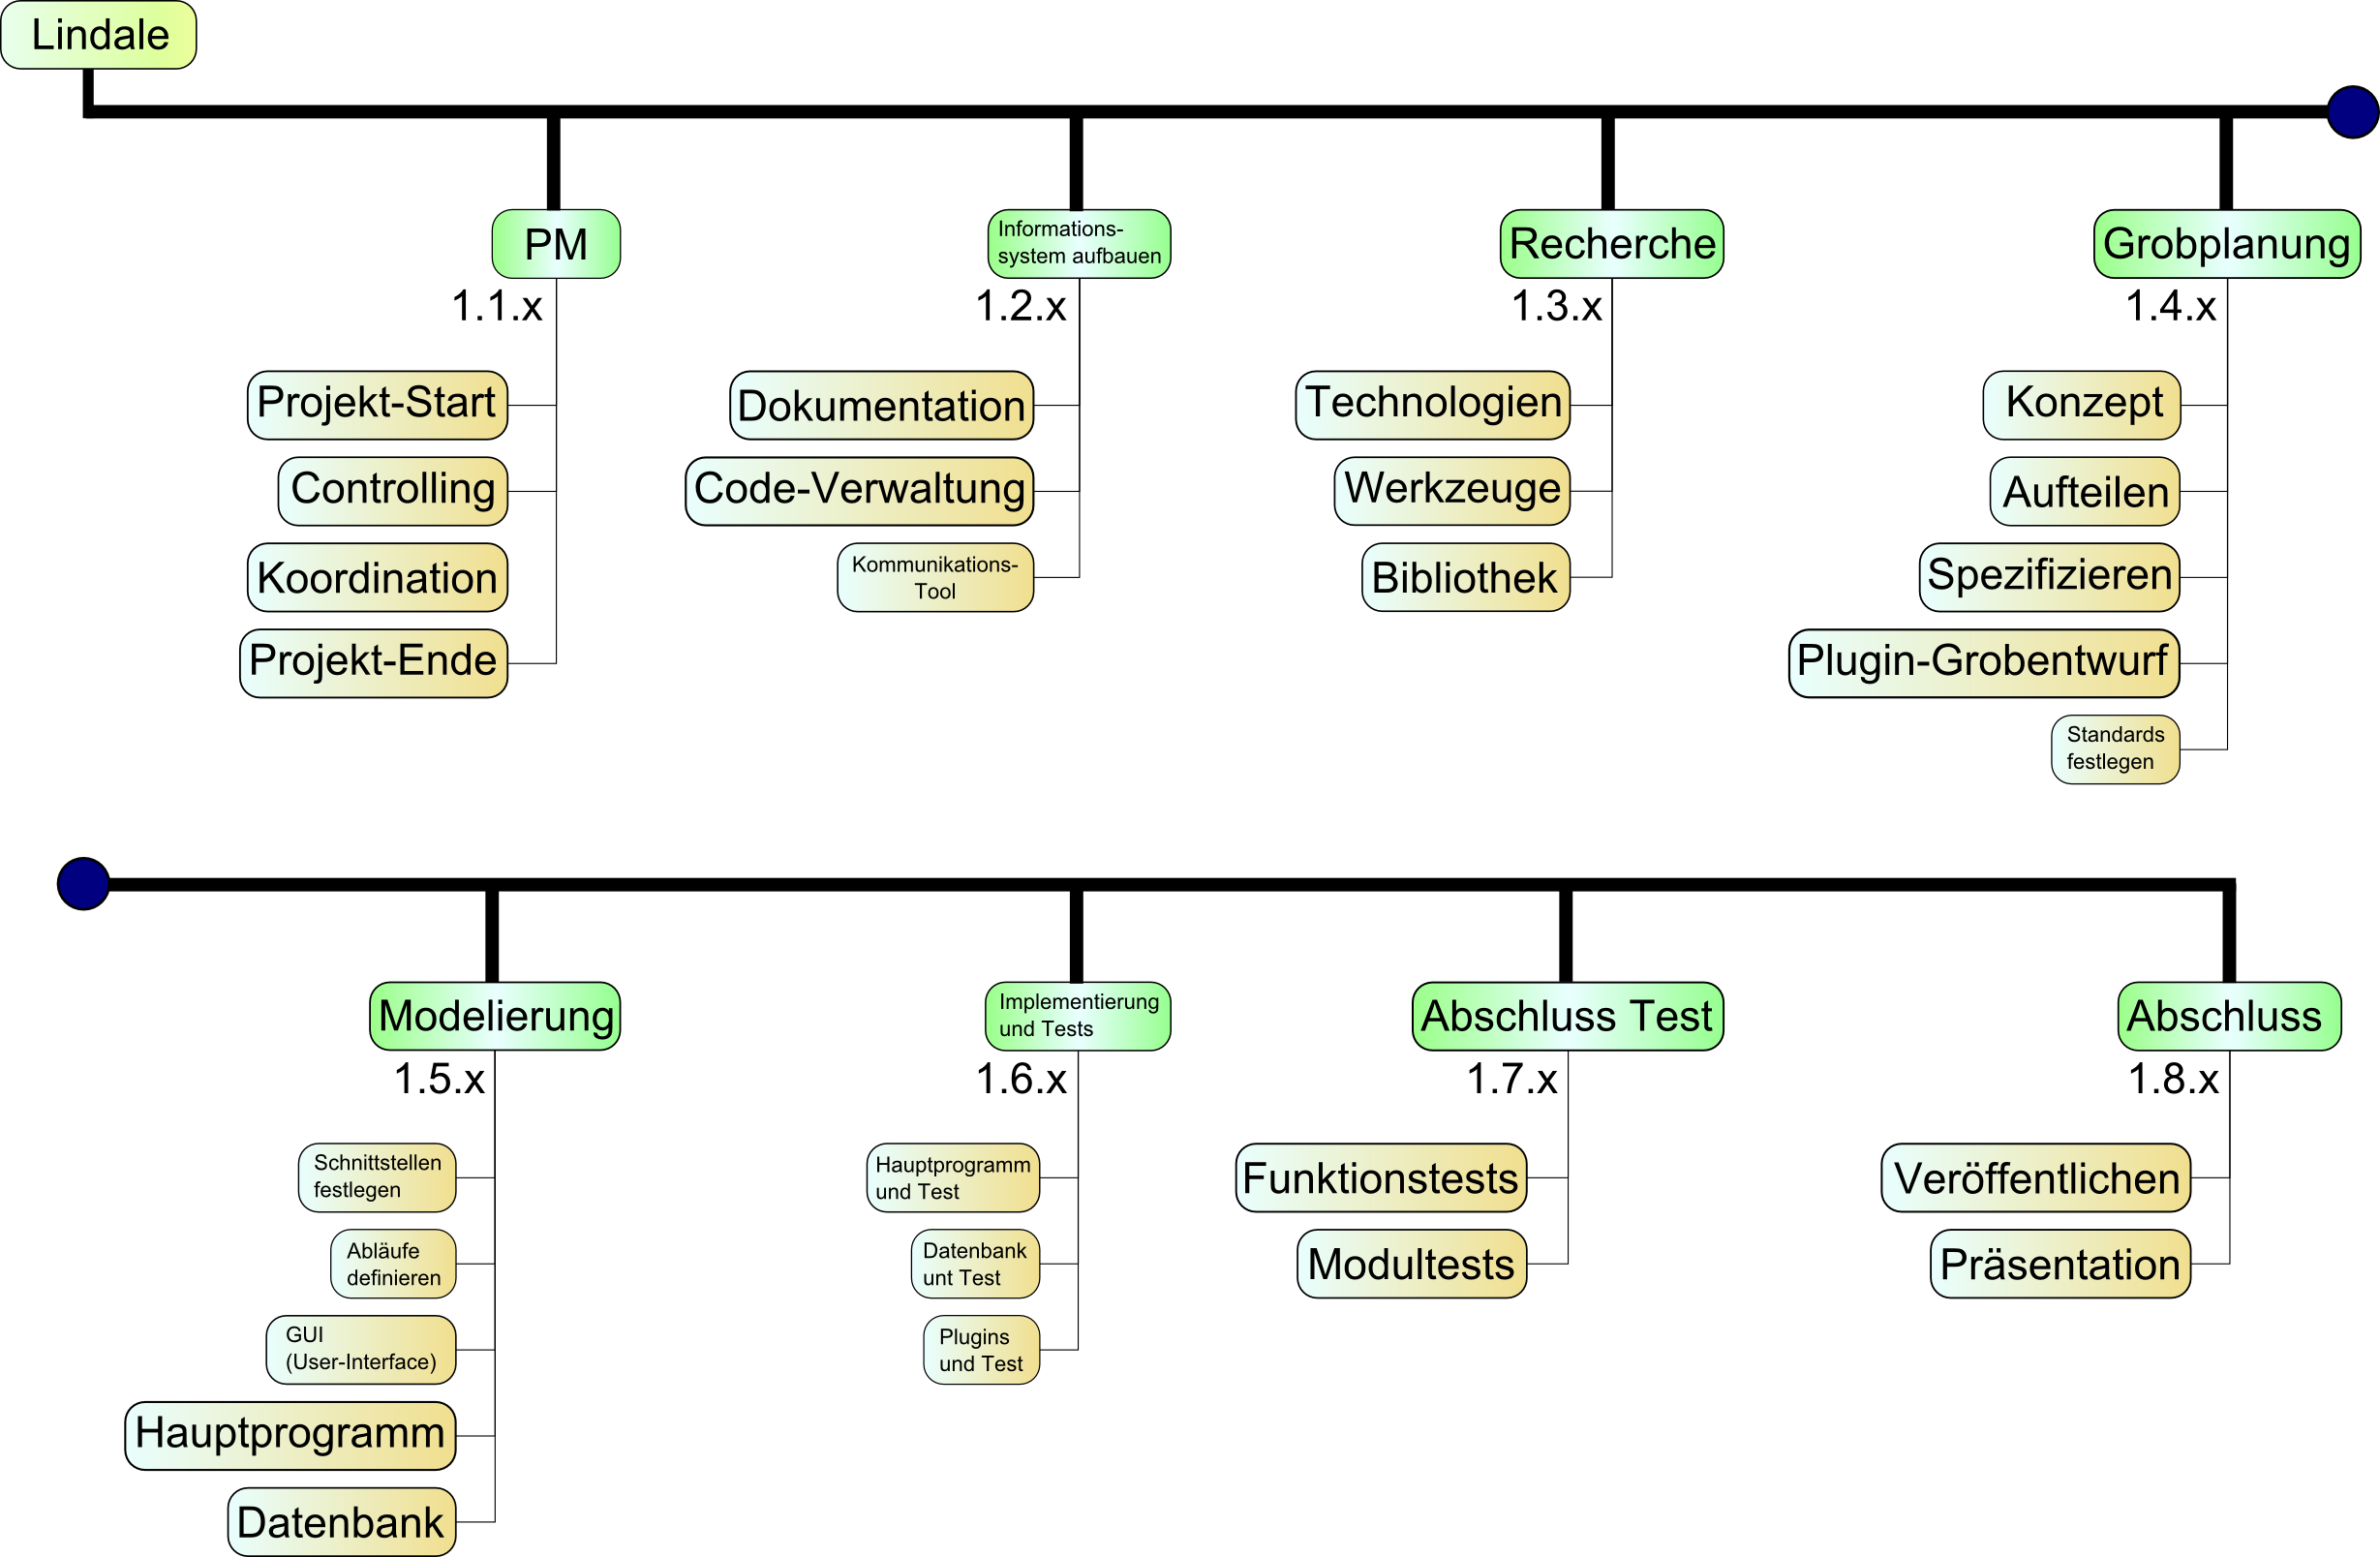
\includegraphics[width=\textwidth, height=\textheight, keepaspectratio, angle=0]{images/psp}
\caption{Projektstrukturplan}
\end{figure}
		\newpage
		\subsection{Arbeitspakete Spezifikation}
%Informationssystem aufbauen
\begin{table}[!ht]
\centering
\small
\tabulinesep=1.4mm
\begin{tabu}{|l|l|}
\hline
\multicolumn{2}{|l|}{ \large \bfseries Informationssystem aufbauen } \\
\end{tabu}
\begin{tabu}{|l|l|}
\hline
\multicolumn{2}{|l|}{  \bfseries Dokumentation (1.2.1) } \\
\hline
\multicolumn{1}{|l|}{ Vorgehensweise / Inhalte } & \multicolumn{1}{|l|}{
\parbox{8.5cm}{
\begin{itemize}
	   \item Linksammlung
	   \item Projektdokumentation
	   \item Protokolle
	   \item Dateien, die während des Projekts erstellt werden, sammeln
	   \item Recherche Ergebnisse
	\end{itemize}
}
} \\
\hline
\multicolumn{1}{|l|}{ Ergebnisse } & \multicolumn{1}{|l|}{
\parbox{8.5cm}{
	\begin{itemize}
	   \item Durchgehende Dokumentation
	   \item Einheitlicher Informationsstand
	\end{itemize}
}
} \\
\end{tabu}
\begin{tabu}{|l|l|}
\hline
\multicolumn{2}{|l|}{  \bfseries Code-Verwaltung (1.2.2) } \\
\hline
\multicolumn{1}{|l|}{ Vorgehensweise / Inhalte } & \multicolumn{1}{|l|}{
\parbox{8.5cm}{
	\begin{itemize}
	   \item Code Versionsverwaltung (mit GIT)
	   \item Commiten / Teamwork sammeln
	   \item Recherche Ergebnisse
	\end{itemize}
}
} \\
\hline
\multicolumn{1}{|l|}{ Ergebnisse } & \multicolumn{1}{|l|}{
\parbox{8.5cm}{
	\begin{itemize}
	   \item Separat an verschiedenen oder gleichen Codestücken arbeiten
	   \item Nicht beeinflussen durch separate Entwicklungsschritte
	\end{itemize}
}
} \\
\end{tabu}
\begin{tabu}{|l|l|}
\hline
\multicolumn{2}{|l|}{  \bfseries Kommunikations-Tool (1.2.3) } \\
\hline
\multicolumn{1}{|l|}{ Vorgehensweise / Inhalte } & \multicolumn{1}{|l|}{
\parbox{8.5cm}{
	\begin{itemize}
	   \item Facebook-Gruppe
	   \item Facebook-Gruppen-Chat
	\end{itemize}
}
} \\
\hline
\multicolumn{1}{|l|}{ Ergebnisse } & \multicolumn{1}{|l|}{
\parbox{8.5cm}{
	\begin{itemize}
	   \item Absprachen, Treffen, Neuigkeiten
	   \item Schneller Informationsaustausch
	\end{itemize}
}
} \\
\hline
\end{tabu}
\end{table}
%Recherche
\begin{table}[!ht]
\centering
\small
\tabulinesep=1.4mm
\begin{tabu}{|l|l|}
\hline
\multicolumn{2}{|l|}{ \large \bfseries Recherche } \\
\end{tabu}
\begin{tabu}{|l|l|}
\hline
\multicolumn{2}{|l|}{  \bfseries Technologien (1.3.1) } \\
\hline
\multicolumn{1}{|l|}{ Vorgehensweise / Inhalte } & \multicolumn{1}{|l|}{
\parbox{8.5cm}{
	\begin{itemize}
	   \item Abschätuen des Implementierungsaufwand
	   \item Moderner Technologien Einsatz (FXML, JavaFX)
	\end{itemize}
}
} \\
\hline
\multicolumn{1}{|l|}{ Ergebnisse } & \multicolumn{1}{|l|}{
\parbox{8.5cm}{
	\begin{itemize}
	   \item Effiziente Implementierung
	   \item Richtiger Einsatz der Technologie
	\end{itemize}
}
} \\
\end{tabu}
\begin{tabu}{|l|l|}
\hline
\multicolumn{2}{|l|}{  \bfseries Werkzeuge (1.3.2) } \\
\hline
\multicolumn{1}{|l|}{ Vorgehensweise / Inhalte } & \multicolumn{1}{|l|}{
\parbox{8.5cm}{
	\begin{itemize}
	   \item Ermitteln von nützlichen Tools
	   \item Ausprobieren der Werkzeuge
	   \item Dokumentieren
	   \item Auswahltreffen
	\end{itemize}
}
} \\
\hline
\multicolumn{1}{|l|}{ Ergebnisse } & \multicolumn{1}{|l|}{
\parbox{8.5cm}{
	\begin{itemize}
	   \item Erfahrungen sammeln
	   \item Geeignete Tools finden
	\end{itemize}
}
} \\
\end{tabu}
\begin{tabu}{|l|l|}
\hline
\multicolumn{2}{|l|}{  \bfseries Bibliothek (1.3.3) } \\
\hline
\multicolumn{1}{|l|}{ Vorgehensweise / Inhalte } & \multicolumn{1}{|l|}{
\parbox{8.5cm}{
	\begin{itemize}
	   \item Suchen
	   \item Experimentieren
	   \item Auswahltreffen
	\end{itemize}
}
} \\
\hline
\multicolumn{1}{|l|}{ Ergebnisse } & \multicolumn{1}{|l|}{
\parbox{8.5cm}{
	\begin{itemize}
	   \item Erleichterte Programmierung
	   \item Richtiger Einsatz der Bibliotheken
	\end{itemize}
}
} \\
\hline
\end{tabu}
\end{table}
%Grobplanung
\begin{table}[!ht]
\centering
\small
\tabulinesep=1.4mm
\begin{tabu}{|l|l|}
\hline
\multicolumn{2}{|l|}{ \large \bfseries Grobplanung } \\
\end{tabu}
\begin{tabu}{|l|l|}
\hline
\multicolumn{2}{|l|}{  \bfseries Aufteilung (1.4.1) } \\
\hline
\multicolumn{1}{|l|}{ Vorgehensweise / Inhalte } & \multicolumn{1}{|l|}{
\parbox{8.5cm}{
	\begin{itemize}
	   \item Aufsplitten der Module
	   \begin{itemize}
	     \item Startprogramm
	     \item GUI
	     \item Plugin-Manager
	     \item Datenbank
	     \item Plugins
	   \end{itemize}
	\end{itemize}
}
} \\
\hline
\multicolumn{1}{|l|}{ Ergebnisse } & \multicolumn{1}{|l|}{
\parbox{8.5cm}{
	\begin{itemize}
	   \item Leichtere Verteilung der Aufgaben
	\end{itemize}
}
} \\
\end{tabu}
\begin{tabu}{|l|l|}
\hline
\multicolumn{2}{|l|}{  \bfseries Spezifizieren (1.4.2) } \\
\hline
\multicolumn{1}{|l|}{ Vorgehensweise / Inhalte } & \multicolumn{1}{|l|}{
\parbox{8.5cm}{
	\begin{itemize}
	   \item Tests definieren
	   \item API / Plugin-API
	   \item SQL-Wrapper
	\end{itemize}
}
} \\
\hline
\multicolumn{1}{|l|}{ Ergebnisse } & \multicolumn{1}{|l|}{
\parbox{8.5cm}{
	\begin{itemize}
	   \item Einheitliche Schnittstellen
	\end{itemize}
}
} \\
\end{tabu}
\begin{tabu}{|l|l|}
\hline
\multicolumn{2}{|l|}{  \bfseries Plugin-Grobentwurf (1.4.3) } \\
\hline
\multicolumn{1}{|l|}{ Vorgehensweise / Inhalte } & \multicolumn{1}{|l|}{
\parbox{8.5cm}{
	\begin{itemize}
	   \item Arten definieren
	   \item Start-/Stop-/Instalations-/Deinstalations- Verhalten definieren
	   \item Modi (Automatisch/Manuel)
	   \item Zugriffe / Zugriffsarten
	   \item Bereitstellung
	\end{itemize}
}
} \\
\hline
\multicolumn{1}{|l|}{ Ergebnisse } & \multicolumn{1}{|l|}{
\parbox{8.5cm}{
	\begin{itemize}
	   \item Modulare Architektur
	\end{itemize}
}
} \\
\end{tabu}
\begin{tabu}{|l|l|}
\hline
\multicolumn{2}{|l|}{  \bfseries Standards festlegen (1.4.4) } \\
\hline
\multicolumn{1}{|l|}{ Vorgehensweise / Inhalte } & \multicolumn{1}{|l|}{
\parbox{8.5cm}{
	\begin{itemize}
	   \item Coding-Standards
	   \item Sprach-Standards
	   \item Formatierungs-Standards
	\end{itemize}
}
} \\
\hline
\multicolumn{1}{|l|}{ Ergebnisse } & \multicolumn{1}{|l|}{
\parbox{8.5cm}{
	\begin{itemize}
	   \item Vereinheitlichung der Entwicklung
	\end{itemize}
}
} \\
\hline
\end{tabu}
\end{table}
%Modellierung
\begin{table}[!ht]
\centering
\small
\tabulinesep=1.4mm
\begin{tabu}{|l|l|}
\hline
\multicolumn{2}{|l|}{ \large \bfseries Modellierung } \\
\end{tabu}
\begin{tabu}{|l|l|}
\hline
\multicolumn{2}{|l|}{  \bfseries Schnittstellen festlegen (1.5.1) } \\
\hline
\multicolumn{1}{|l|}{ Vorgehensweise / Inhalte } & \multicolumn{1}{|l|}{
\parbox{8.5cm}{
	\begin{itemize}
	   \item UML (Klassen-Diagramm) Modellierung
	   \item APIs Implementierungs nah definieren
	   \begin{itemize}
	     \item Plugin-API
	     \item Interne API
	     \begin{itemize}
			\item SQL-Execution
			\item GUI
		 \end{itemize}
	   \end{itemize}
	   \item Testfälle definieren
	\end{itemize}
}
} \\
\hline
\multicolumn{1}{|l|}{ Ergebnisse } & \multicolumn{1}{|l|}{
\parbox{8.5cm}{
	\begin{itemize}
	   \item Implementierungsnahes Model
	   \item Testdefinitionen
	\end{itemize}
}
} \\
\end{tabu}
\begin{tabu}{|l|l|}
\hline
\multicolumn{2}{|l|}{  \bfseries Abläufe definieren (1.5.2) } \\
\hline
\multicolumn{1}{|l|}{ Vorgehensweise / Inhalte } & \multicolumn{1}{|l|}{
\parbox{8.5cm}{
	\begin{itemize}
	   \item UML (Sequenz-Diagramm)
	   \item Flussdiagramme
	   \item Programmstart
	   \item Plugin: Start-/Stop-/Instalations-/Deinstalations-Verhalten
	   \item Quellen Hinzufügen
	   \item Datenbankzugriffe (Wrapper ↔ SQLite)
	   \item Medien laden / abspielen
	   \item Laden von Plugins in die GUI
	   \item Fehlermeldungen
	\end{itemize}
}
} \\
\hline
\multicolumn{1}{|l|}{ Ergebnisse } & \multicolumn{1}{|l|}{
\parbox{8.5cm}{
	\begin{itemize}
	   \item Definierter Programmablauf
	\end{itemize}
}
} \\
\hline
\end{tabu}
\end{table}
\begin{table}[!ht]
\centering
\small
\tabulinesep=1.4mm
\begin{tabu}{|l|l|}
\hline
\multicolumn{2}{|l|}{  \bfseries GUI (1.5.3) } \\
\hline
\multicolumn{1}{|l|}{ Vorgehensweise / Inhalte } & \multicolumn{1}{|l|}{
\parbox{8.5cm}{
	\begin{itemize}
	   \item Grafische Modelierung
	   \item Dialoge Modellieren / Festlegen
	   \item Aussehen (Farbe, Steuerelemente, Schnittstellen zum User)
	\end{itemize}
}
} \\
\hline
\multicolumn{1}{|l|}{ Ergebnisse } & \multicolumn{1}{|l|}{
\parbox{8.5cm}{
	\begin{itemize}
	   \item Strukturierte und moderne Oberfläche
	\end{itemize}
}
} \\
\end{tabu}
\begin{tabu}{|l|l|}
\hline
\multicolumn{2}{|l|}{  \bfseries Hauptprogramm (1.5.4) } \\
\hline
\multicolumn{1}{|l|}{ Vorgehensweise / Inhalte } & \multicolumn{1}{|l|}{
\parbox{8.5cm}{
	\begin{itemize}
	   \item UML (Klassen-Diagramme)
	   \item Schnittstellen zu Bibliotheken
	   \item Schnittstellen zur Datenbank
	   \item Statement-Exekution-Parser
	\end{itemize}
}
} \\
\hline
\multicolumn{1}{|l|}{ Ergebnisse } & \multicolumn{1}{|l|}{
\parbox{8.5cm}{
	\begin{itemize}
	   \item Ein Model des Hauptprogrammes
	\end{itemize}
}
} \\
\end{tabu}
\begin{tabu}{|l|l|}
\hline
\multicolumn{2}{|l|}{  \bfseries Datenbank (1.5.5) } \\
\hline
\multicolumn{1}{|l|}{ Vorgehensweise / Inhalte } & \multicolumn{1}{|l|}{
\parbox{8.5cm}{
	\begin{itemize}
	   \item E3R-Methode
	   \item 5. Normalform
	   \item Seminar Wenzel
	   \item Test-Transaktionen definieren
	\end{itemize}
}
} \\
\hline
\multicolumn{1}{|l|}{ Ergebnisse } & \multicolumn{1}{|l|}{
\parbox{8.5cm}{
	\begin{itemize}
	   \item Datenbankmodel nahe Implementierung
	   \item Testdefinitionen
	\end{itemize}
}
} \\
\hline
\end{tabu}
\end{table}
%Implementierung und Tests
\begin{table}[!ht]
\centering
\small
\tabulinesep=1.4mm
\begin{tabu}{|l|l|}
\hline
\multicolumn{2}{|l|}{ \large \bfseries Implementierung und Tests } \\
\end{tabu}
\begin{tabu}{|l|l|}
\hline
\multicolumn{2}{|l|}{  \bfseries Hauptprogramm und Test (1.6.1) } \\
\hline
\multicolumn{1}{|l|}{ Vorgehensweise / Inhalte } & \multicolumn{1}{|l|}{
\parbox{8.5cm}{
	\begin{itemize}
	   \item Umsetzen der Klassen-Diagramm (Dummys)
	   \item Umsetzung definierter Test (JUnit)
	   \item Implementierung der Funktionalität
	   \item GUI-Test
	\end{itemize}
}
} \\
\hline
\multicolumn{1}{|l|}{ Ergebnisse } & \multicolumn{1}{|l|}{
\parbox{8.5cm}{
	\begin{itemize}
	   \item Lauffähiges Hauptprogramm (nicht mehr grabbeln)
	\end{itemize}
}
} \\
\end{tabu}
\begin{tabu}{|l|l|}
\hline
\multicolumn{2}{|l|}{  \bfseries Datenbank und Test (1.6.2) } \\
\hline
\multicolumn{1}{|l|}{ Vorgehensweise / Inhalte } & \multicolumn{1}{|l|}{
\parbox{8.5cm}{
	\begin{itemize}
	   \item Implementieren
	   \item Abfragen Tests / Transaktions Tests
	\end{itemize}
}
} \\
\hline
\multicolumn{1}{|l|}{ Ergebnisse } & \multicolumn{1}{|l|}{
\parbox{8.5cm}{
	\begin{itemize}
	   \item Super Datenbank
	\end{itemize}
}
} \\
\end{tabu}
\begin{tabu}{|l|l|}
\hline
\multicolumn{2}{|l|}{  \bfseries Plugins und Test (1.6.3) } \\
\hline
\multicolumn{1}{|l|}{ Vorgehensweise / Inhalte } & \multicolumn{1}{|l|}{
\parbox{8.5cm}{
	\begin{itemize}
	   \item Implementieren
	   \item Testen
	   \item Schnittstellen Tests
	\end{itemize}
}
} \\
\hline
\multicolumn{1}{|l|}{ Ergebnisse } & \multicolumn{1}{|l|}{
\parbox{8.5cm}{
	\begin{itemize}
	   \item Funktionierende Plugins
	\end{itemize}
}
} \\
\hline
\end{tabu}
\end{table}
%Abschluss Test
\begin{table}[!ht]
\centering
\small
\tabulinesep=1.4mm
\begin{tabu}{|l|l|}
\hline
\multicolumn{2}{|l|}{ \large \bfseries Abschluss Test } \\
\end{tabu}
\begin{tabu}{|l|l|}
\hline
\multicolumn{2}{|l|}{  \bfseries Funktionstests (1.7.1) } \\
\hline
\multicolumn{1}{|l|}{ Vorgehensweise / Inhalte } & \multicolumn{1}{|l|}{
\parbox{8.5cm}{
	\begin{itemize}
	   \item Alle Funktionalitäten überprüfen
	   \item Fehler provozieren
	\end{itemize}
}
} \\
\hline
\multicolumn{1}{|l|}{ Ergebnisse } & \multicolumn{1}{|l|}{
\parbox{8.5cm}{
	\begin{itemize}
	   \item Programm kann veröffentlicht werden
	\end{itemize}
}
} \\
\end{tabu}
\begin{tabu}{|l|l|}
\hline
\multicolumn{2}{|l|}{  \bfseries Modultests (1.7.2)) } \\
\hline
\multicolumn{1}{|l|}{ Vorgehensweise / Inhalte } & \multicolumn{1}{|l|}{
\parbox{8.5cm}{
	\begin{itemize}
	   \item Jedes Modul separatem Test unterzogen
	   \item Modulgruppen testen
	   \item Teil-Programm-Tests z.B.: Hauptprogramm
	\end{itemize}
}
} \\
\hline
\multicolumn{1}{|l|}{ Ergebnisse } & \multicolumn{1}{|l|}{
\parbox{8.5cm}{
	\begin{itemize}
	   \item Funktionalität der Programmteile gewährleistet
	\end{itemize}
}
} \\
\hline
\end{tabu}
\end{table}
%Abschluss
\begin{table}[!ht]
\centering
\small
\tabulinesep=1.4mm
\begin{tabu}{|l|l|}
\hline
\multicolumn{2}{|l|}{ \large \bfseries Abschluss } \\
\end{tabu}
\begin{tabu}{|l|l|}
\hline
\multicolumn{2}{|l|}{  \bfseries Veröffentlichen (1.8.1) } \\
\hline
\multicolumn{1}{|l|}{ Vorgehensweise / Inhalte } & \multicolumn{1}{|l|}{
\parbox{8.5cm}{
	\begin{itemize}
	   \item Lizenzfrage klären
	   \item Webpräsenz
	   \item Webhoster finden
	\end{itemize}
}
} \\
\hline
\multicolumn{1}{|l|}{ Ergebnisse } & \multicolumn{1}{|l|}{
\parbox{8.5cm}{
	\begin{itemize}
	   \item Veröffentlichen
	\end{itemize}
}
} \\
\end{tabu}
\begin{tabu}{|l|l|}
\hline
\multicolumn{2}{|l|}{  \bfseries Präsentieren (1.8.2) } \\
\hline
\multicolumn{1}{|l|}{ Vorgehensweise / Inhalte } & \multicolumn{1}{|l|}{
\parbox{8.5cm}{
	\begin{itemize}
	   \item Projekthandbuch
	   \item Präsentation vorbereiten / üben / halten
	\end{itemize}
}
} \\
\hline
\multicolumn{1}{|l|}{ Ergebnisse } & \multicolumn{1}{|l|}{
\parbox{8.5cm}{
	\begin{itemize}
	   \item Präsentations Note
	\end{itemize}
}
} \\
\hline
\end{tabu}
\end{table}

	\clearpage
	\section{Terminplan}
			%Table Head Macro
\newcommand*{\thead}[1]{\multicolumn{4}{|c|}{\bfseries #1}}

\subsection{Projektmeilensteinplan}
\begin{table}[!ht]
\caption{Projektmeilensteinplan}
\centering
\tabulinesep=1.4mm
\begin{tabu}{|l|l|l|l|}
\hline
\thead{Projektmeilensteinplan} \\
\hline
{\bf PSP-Code} & {\bf Meilenstein} & {\bf Plantermin} & {\bf Isttermin} \\
\hline
& Projektstart & 05.10.2013 & 05.10.2013 \\
\hline
1.3 & Start Recherche & 06.10.2013 &  06.10.2013 \\
\hline
1.4 & Grobplannung & 05.10.2013 & 05.10.2013 \\
\hline
1.4.1 & Konzeptions beginn & 21.11.2013 & 21.11.2013 \\
\hline
1.6 & Modellierung & 06.12.2013 & \textcolor{red}{ 09.12.2013 } \\
\hline
1.7.1 & Start Hauptprogramm Entwicklung & 07.12.2013 & \textcolor{red}{ 15.12.2013 }\\
\hline
1.7.2 & Beginn Plugin-Entwicklung & 21.12.2013 & \\
\hline
1.8  & Start Testen & 06.12.2013 & \\
\hline
1.9 & Projektabschluss & 10.01.2013 & \\
\hline
\end{tabu}
\end{table}

		\newpage
		%Table Head Macro
\newcommand*{\theadGE}[1]{\multicolumn{5}{|c|}{\bfseries #1}}

\subsection{Projekt-Resourcen-Zeitplan}
\begin{table}[!ht]
\caption{Projekt-Resourcen-Zeitplan}
\centering
\begin{tabu}{|l|l|c|c|c|}
\hline

\theadGE{Projekt-Resourcen-Zeitplan} \\
\hline
\hline
{\parbox{2cm}{\bf PSP-Code       }} &
{\parbox{3cm}{\bf Arbeitspaket   }} &
{\parbox{1.7cm}{\bf Jochen Morent  }} &
{\parbox{1.7cm}{\bf Jeremias Eppler}} &
{\parbox{1.7cm}{\bf Georgi Georgiev}}\\
\hline

1.2 & \multicolumn{4}{c|}{\bf Informationssystem aufbauen }  \\
\hline
\rowfont{\scriptsize}
1.2.1 & Dokumentation & 5 & 5 & 5\\
\hline
\rowfont{\scriptsize}
1.2.2 & Code Verwaltung & 3 &  & \\
\hline
\rowfont{\scriptsize}
1.2.3 & Kommunikationstool &  & 3  & \\
\hline

1.3 & \multicolumn{4}{c|}{\bf Recherche} \\
\hline
\rowfont{\scriptsize}
1.3.1 & Technologien & 5 & 5 & 5 \\
\hline
\rowfont{\scriptsize}
1.3.2 & Werkzeuge & 5 & 5 & 5 \\
\hline
\rowfont{\scriptsize}
1.3.3 & Bibliothek & 5 & 5 & 5 \\
\hline

1.4 & \multicolumn{4}{c|}{\bf Grobplanung} \\
\hline
\rowfont{\scriptsize}
1.4.1 & Konzept & 2 & 2 & 2 \\
\hline
\rowfont{\scriptsize}
1.4.2 & Aufteilen & 1 & 1 & 1 \\
\hline
\rowfont{\scriptsize}
1.4.3 & Spezifizieren & 5 & 5 & 5 \\
\hline
\rowfont{\scriptsize}
1.4.4 & Plugin-Grobentwurf & 5 & 5 & 5 \\
\hline
\rowfont{\scriptsize}
1.4.5 & Standards festlegen & 1 &  &  \\
\hline

1.5 & \multicolumn{4}{c|}{\bf Modelierung} \\
\hline
\rowfont{\scriptsize}
1.5.1 & Schnittstellen festlegen & 3 & 2 & 2 \\
\hline
\rowfont{\scriptsize}
1.5.2 & Abläufe definieren & 2 & 2 & 2 \\
\hline
\rowfont{\scriptsize}
1.5.3 & GUI & 5 & 5 & 6 \\
\hline
\rowfont{\scriptsize}
1.5.4 & Hauptprogramm & 4 & 3 & 3 \\
\hline
\rowfont{\scriptsize}
1.5.5 & Datenbank & 6 & 6 & 6 \\
\hline

1.6 & \multicolumn{4}{c|}{\bf Implementierung und Tests} \\
\hline
\rowfont{\scriptsize}
1.6.1 & Hauptprogramm und Test & 10 & 10 & 10 \\
\hline
\rowfont{\scriptsize}
1.6.2 & Datenbank und Test & 3 & 3 &  \\
\hline
\rowfont{\scriptsize}
1.6.3 & Plugins und Test & 12 & 12 & 12 \\
\hline

1.7 & \multicolumn{4}{c|}{\bf Abschlusstest} \\
\hline
\rowfont{\scriptsize}
1.7.1 & Funktionstest & 6 & 6 & 6 \\
\hline
\rowfont{\scriptsize}
1.7.2 & Modultest & 8 & 8 & 8 \\
\hline

1.8 & \multicolumn{4}{c|}{\bf Abschluss} \\
\hline
\rowfont{\scriptsize}
1.8.1 & Veröffentlichen & 10 & 10 & 10 \\
\hline
\rowfont{\scriptsize}
1.8.1 & Präsentation & 2 & 2 & 2 \\
\hline

\end{tabu}
\end{table}

		\newpage
		\subsection{Projektbalkenplan}
\begin{figure}[!ht]
\center
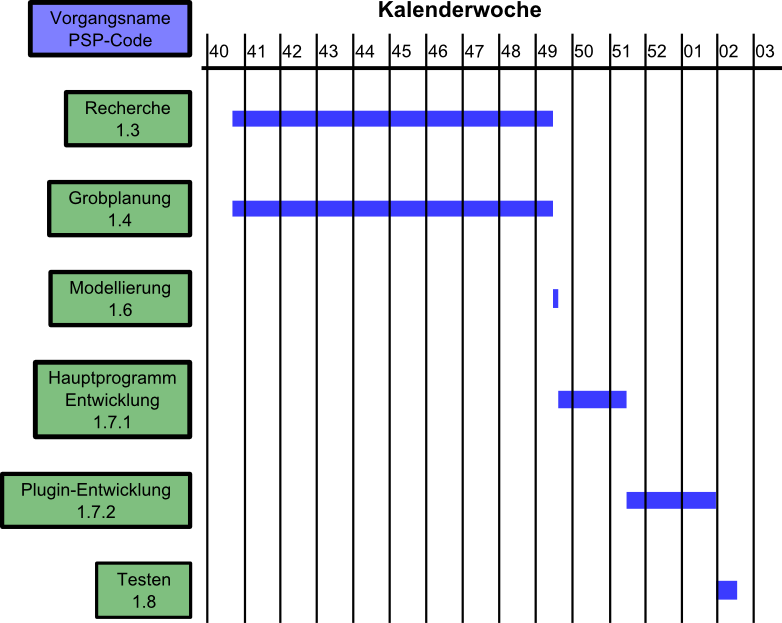
\includegraphics[width=\linewidth]{images/balkenplan}
\caption{Projektbalkenplan}
\end{figure}


%-----------------------------------------------
%  Projektcontrolling
%-----------------------------------------------
\newpage
\chapter{Projektcontrolling}
	\section{Projektfortschrittsbericht}
\noindent
%vspace between the lines
\tabulinesep=1.3mm
\begin{longtabu} to \linewidth {|X[c]|X[c]|X[c]|X[c]|X[c]|}
\hline 
\rowfont{\large}
\multicolumn{5}{|c|}{ Lindale Projektfortschrittsbericht} \\ 
\hline 
sehr gut & gut \checkmark & okay & schlecht & sehr schlecht \\ 
\hline 
\multicolumn{5}{|l|}{ \bfseries Gestamtstatus des Projektes } \\ 
\hline 
\multicolumn{5}{|l|}{
\parbox{15cm}{ 
	\begin{itemize}
	   \item Projekt liegt im Zeitrahmen
	   \item Hinzugekommenes Know-how durch Datenbankprogrammierungs Lehrveranstaltung und Seminar
	   \item Angespannte Arbeitssituation aller Teammitglieder
	   \item Verteilung von Inhalten des Projekthandbuches → Informations und Datenmisstand innerhalb des Projektes
	\end{itemize}
}
} \\
\hline 
\multicolumn{5}{|l|}{ \bfseries Status: Projektziele und Betrachtungsobjekte } \\ 
\hline 
\multicolumn{5}{|l|}{
\parbox{15cm}{
	\begin{itemize}
	   \item Zieladaptierung: weglassen von Features wie:
	   \begin{itemize}
	     \item Logische und Physikalische Collection
	     \item Bewertungssystem
	   \end{itemize}
	   \item Adaptierung der Nebenziele war notwendig dennoch $\rightarrow$ Status: \gut
	\end{itemize}
}
} \\
\hline
\multicolumn{5}{|l|}{ \bfseries Status: Projektleistungsfortschritt } \\ 
\hline 
\multicolumn{5}{|l|}{
\parbox{15cm}{
    \begin{itemize}
      \item Arbeitspakete fortschritt:
     
	  \begin{description}
	     \item[1.2] Erfolgreich umgesetzt
	     \item[1.3] Recherche für die Hauptprogramm Entwicklung abgeschlossen
	     \item[1.4.3] Spezifizieren für die Entwicklung des Hauptprogramms abgeschlossen
	     \item[1.4.5] Standards soweit festgelegt, das entwickelt werden kann
	     \item[1.5.5] Datenbank Modellierung abgeschlossen
	  \end{description}
	  
	  \item Verzug mit dem modellieren der GUI des Hauptprogrammes $\rightarrow$ Status: \okay
	\end{itemize}
  }
} \\
\hline 
\multicolumn{5}{|l|}{\bfseries Status: Projekttermine } \\ 
\hline 
\multicolumn{5}{|l|}{
\parbox{15cm}{
	\begin{itemize}
	   \item Verzögerung bei der Entwicklung und Modellierung des Hauptprogramms durch neu hinzugewonnenes Wissen
	   \item Wegen Verzögerung beim modellieren $\rightarrow$ Status: \okay
	\end{itemize}
  }
} \\
\hline 
\multicolumn{5}{|l|}{ \bfseries Status: Projektumwelt, Beziehungen zu anderen Projekten } \\ 
\hline 
\multicolumn{5}{|l|}{
\parbox{15cm}{
	\begin{itemize}
	   \item Hinzugekommener Dozent als Experte zwischen Datenbank und Anwendungsprogramm
	   \item Starke Wissenserweiterung $\rightarrow$ Status: \sehrGut
	\end{itemize}
}
} \\
\hline 
\multicolumn{5}{|l|}{ \bfseries Status: Maßnahmen } \\ 
\hline 
\multicolumn{5}{|l|}{
\parbox{15cm}{
	\begin{itemize}
	  \item Adaptieren der Nebenziele
	  \item Neu ausrichtung des Projektes mithilfe des gewonnenen Informationen
	  \item Zusammenführen der Projekthandbuch Informationen
	  \item Einpflegen von Informationen in das Informationssystem
	  \item Information aller Teammitglieder und Umsetzung läuft $\rightarrow$ Status: \sehrGut
	\end{itemize}
}
} \\
\hline 
\multicolumn{5}{|l|}{ \bfseries Status: Anhang } \\ 
\hline 
\multicolumn{5}{|l|}{
\parbox{15cm}{
    \begin{itemize}
	   \item Projekt Score Card
	\end{itemize}
}
} \\
\hline 
\multicolumn{1}{|l}{Version 1.1} & \multicolumn{2}{l}{Datum 6 Dez, 2013} & \multicolumn{2}{l|}{Ersteller: Lindale-Team } \\
\hline

\end{longtabu}

	% \clearpage
	\section{Projekt-Score-Card}
\begin{figure}[!ht]
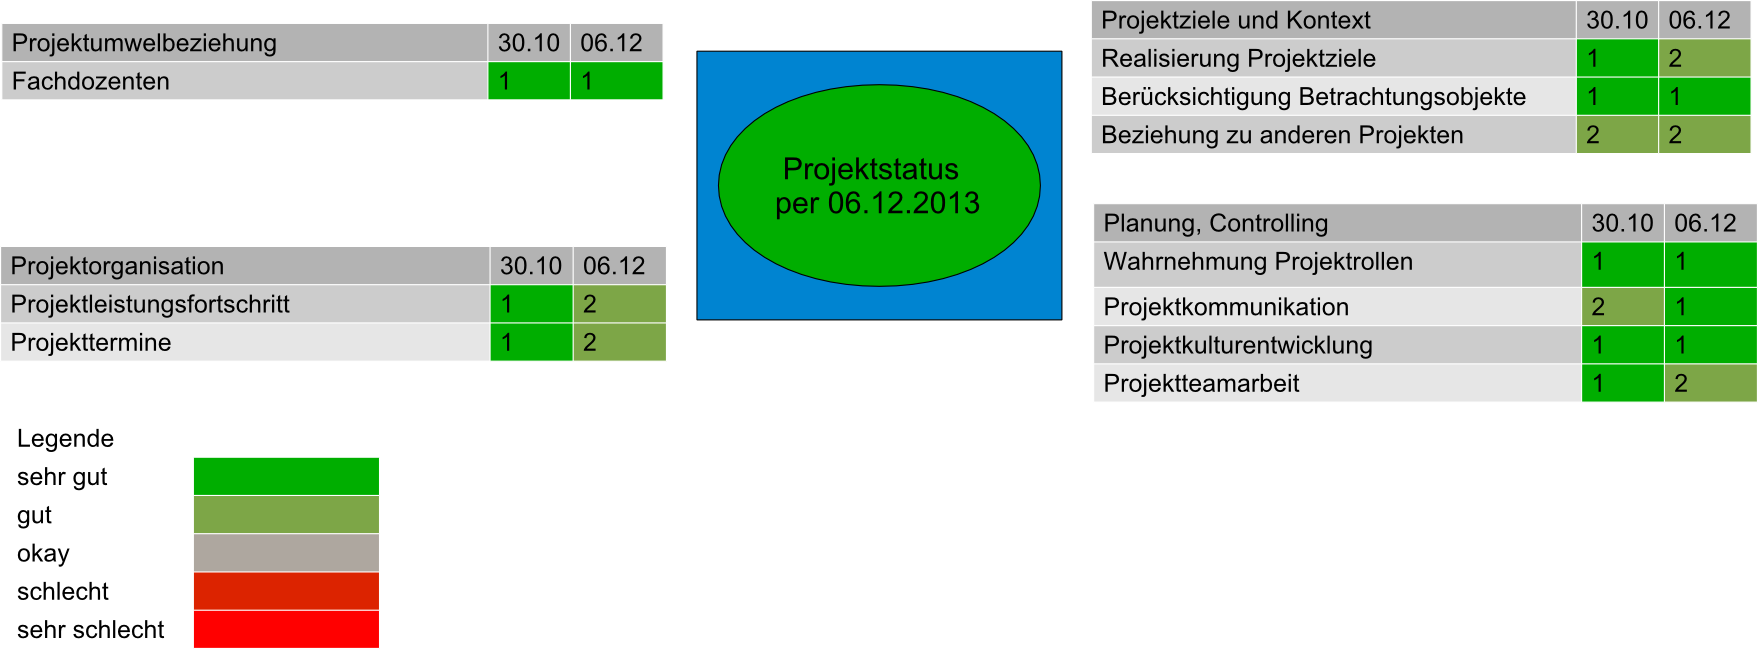
\includegraphics[width=\textwidth, height=\textheight, keepaspectratio, angle=0]{images/projekt-score-card}
\caption{Projekt-Score-Card}
\end{figure}
	\clearpage
	\section{Projektkommunikationsstrukturen}
\tabulinesep=1.3mm
\begin{longtabu} to 14cm {|X[l]|X[l]|X[l]|X[l]|}
\hline
\parbox{3cm}{Bezeichnung der Sitzung} & \parbox{3cm}{Inhalte} & \parbox{3cm}{Teilnehmer} & \parbox{3cm}{Häufigkeit und Dauer} \\
\hline
\parbox{3cm}{Projektauftraggeber-Sitzung} & \parbox{3cm}{Datenbankentwurf und Implentierung} & \parbox{3cm}{Lindale Team, B. Wenzel F.Reischer} & \parbox{3cm}{Im Data Management - Seminar ungefähr 20 Minuten} \\
\hline
\parbox{3cm}{Projektteamsitzung} & \parbox{3cm}{Besprechung von bis jetzt erledigten Aufgaben (Fortschrittsbericht), Erarbeitung und Besprechung aus dem PSP, Aufgabenverteilung} & \parbox{3cm}{Lindale Team} & \parbox{3cm}{wöchentlich 2 bis 10 Stunden} \\
\hline
\parbox{3cm}{Coaching–Sitzungen} & \parbox{3cm}{Besprechung der Inhalte aus dem Projekthandbuch und der Teamarbeit} & \parbox{3cm}{Lindale Team, M. Meusburger} & \parbox{3cm}{Im Projektmanagement-Seminar ungefähr 20 Minuten} \\
\hline
\end{longtabu}

%-----------------------------------------------
%  Projektabschluss
%-----------------------------------------------
\newpage
\chapter{Projektabschluss}
	\section{Projektabschlussbericht}
\noindent
%vspace between the lines
\tabulinesep=1.3mm
\begin{longtabu} to \linewidth {|X[c]|X[c]|X[c]|X[c]|X[c]|}

\hline 
\rowfont{\large}
\multicolumn{5}{|c|}{ Projektabschlussbericht } \\ 
\hline 
sehr gut & gut \checkmark & okay & schlecht & sehr schlecht \\ 
\hline
  
\multicolumn{5}{|l|}{ \bfseries Gesamteindruck } \\ 
\hline    

\multicolumn{5}{|l|}{
\parbox{15cm}{ 
	\begin{itemize}
	   \item Projektziele nicht alle erreicht
	   \begin{itemize}
	       \item Groplanung und Modellierung abgeschlossen
	       \item Technologien ausgewählt
	   	   \item Entwicklung des Hauptprogramms erreicht
	   \end{itemize}
	   \item Noch nicht erreichte Ziele, wegen Verschiebung einer Klausur
	   \begin{itemize}
	     \item Entwicklung von Plugins
	     \item Testen der gesamten Applikation
	   \end{itemize}
	\end{itemize}
}
} \\
\hline 

\multicolumn{5}{|l|}{ \bfseries Reflexion: Erfüllung der geplanten Leistungen, Einhaltung der geplanten Termine} \\ 
\hline

\multicolumn{5}{|l|}{ 
\parbox{15cm}{
\begin{itemize}
  \item Erreichte Meilensteine
  \begin{itemize}
    \item Grobplanung und Modellierung abgeschlossen
    \item Technologien ausgewählt
    \item Entwicklung des Hauptprogramms mit Verspätung erreicht
  \end{itemize}
  \item Erreichte Leistungen
  \begin{itemize}
    \item viel Wissen durch ausgiebige Recherche erarbeitet
    \item Gute Planung und modellierung der Applikation
    \item Teilweise Implementierung des Projektes
  \end{itemize}
\end{itemize}
}
} \\
\hline

\multicolumn{5}{|l|}{ \bfseries Reflexion: Projektumweltbeziehungen, Beziehungen zu anderen Projekten } \\ 
\hline 
\multicolumn{5}{|l|}{
\parbox{15cm}{
\begin{itemize}
  \item Projektumweltbeziehung
  \begin{itemize}
    \item Die Anzahl der Dozenten hat sich im Verlauf des Projektes von zwei Ansprechpartner auf vier Ansprechpartner erhöht
  \end{itemize}
  \item Beziehung zu anderen Projekten
  \begin{itemize}
    \item Die Entwicklung von Java 8 durch das OpenJDK Projekt verläuft Planmäßig
  \end{itemize}
\end{itemize}
}
} \\
\hline 

\multicolumn{5}{|l|}{ \bfseries Reflexion: Teamarbeit, Einsatz von Projektmanagement } \\ 
\hline 
\multicolumn{5}{|l|}{
\parbox{15cm}{
\begin{itemize}
  \item hoher Einsatz von Projektmanagement Methoden durch Lehrveranstaltung zum Projektmanagement
  \item Projekt unter permanenter Kontrolle aller Teammitglieder
  \item Gute Teamarbeit und Koordinierung durch
  \begin{itemize}
    \item Projektteamleiter
    \item Einsatz von Kommunikationstechnologie
    \item klare Terminregelungen
  \end{itemize}
  \item hoher Wissensaustausch über eigenes Wiki
  \item ausgegliechene Aufgabenverteilung auf alle Mitglieder
  \item insgesamt sehr gute Teamarbeit
\end{itemize}
}
} \\
\hline  

\multicolumn{5}{|l|}{ \bfseries Zusammenfassende Erfahrungen für andere Projekte } \\ 
\hline 

\multicolumn{5}{|l|}{
\parbox{15cm}{
\begin{itemize}
  \item lernen von Projektmanagement Methoden anhand des Projektes kann in Zukunft genutzt werden
  \item Erfahrung mit sehr neuen, teilweise noch im Beta-Stadium befindlicher, Technologien
  \item Datenbank modellierung und programmierung wurde durch LV's erarbeitet
  \item kennen lernen von Git als Code-Versionierungs-Verwaltung für Teams
  \item erste Erfahrung mit Software Engeeniering von größeren Anwendungen
\end{itemize}
}
} \\
\hline 

\multicolumn{1}{|l}{Version 1.0} & \multicolumn{2}{l}{Datum 06 Jan, 2014} & \multicolumn{2}{l|}{Ersteller: Lindale-Team } \\
\hline

%\subsection{Seite 391 Happy Projects!, Roland Gareis, MANZ 2006 }
\end{longtabu}

\end{document}